% This file: 			Prelim. draft for Heckman to see progress
% Contributors: 		Pietro Biroli, Daniela Del Boca, Linor Kiknadze, 
%					Yu Kyung Koh, Sylvi Kuperman, Sidharth Moktan, 
%					Chiara Pronzato, Nirali Trevedi, Anna Ziff
% Original date: 		10/10/16
% Project: 			Reggio Evaluation

\documentclass[12pt]{article}
\usepackage[top=1in, bottom=1in, left=1in, right=1in]{geometry}
\parindent 22pt

\usepackage{adjustbox}
\usepackage{amsmath}
\usepackage{amssymb}
\usepackage{array}
\usepackage{booktabs}
\usepackage{datetime}
\usepackage{fancyhdr}
\usepackage{float}
\usepackage{graphicx}
\usepackage[colorlinks=true,linkcolor=blue,urlcolor=blue,anchorcolor=blue,citecolor=blue]{hyperref}
\usepackage{lscape}
\usepackage{multirow}
\usepackage{natbib}
\usepackage{setspace}
\usepackage{tabularx}
\usepackage[colorinlistoftodos,linecolor=black]{todonotes}
\usepackage{appendix}
\usepackage{pgffor}
\usepackage{caption} 
\usepackage{threeparttable}
\captionsetup[table]{skip=3pt}

\settimeformat{hhmmsstime}

\newcolumntype{L}[1]{>{\raggedright\arraybackslash}p{#1}}
\newcolumntype{C}[1]{>{\centering\arraybackslash}p{#1}}
\newcolumntype{R}[1]{>{\raggedleft\arraybackslash}p{#1}}


\usepackage{sectsty}
\sectionfont{\fontsize{12}{12}\selectfont}
\subsectionfont{\fontsize{12}{12}\selectfont}

\begin{document}

\title{\normalsize \textbf{Evaluation of the Reggio Approach} \\ \normalsize Draft}
\author{\normalsize Reggio Team}
\date{\normalsize Original version: October 3, 2016 \\ Current version: \today}
\maketitle

\doublespacing

This draft presents (i) a brief description of the data, (ii) a simple analysis comparing individuals who attended the Reggio Emilia municipal schools to individuals in Reggio Emilia who did not attend any preschool, and (iii) a discussion of selection into preschool on observed characteristics. 

\section{Data}
\label{sec:data}

The sample is a subset of the individuals in Reggio Emilia, Parma, and Padova who were born in the year ranges of the five cohorts.  These individuals were collected from the population registries in each of the cities. The sample was then restricted to those individuals living in the same city in which they were raised. All cohorts except the youngest one were restricted to individuals who are Italian citizens. In contrast, the youngest cohort includes an oversampling of immigrant children. The sample from Reggio Emilia, across all cohorts, includes an oversampling of those who attended municipal schools, as this is considered the treatment.

Of the reference sample, 7,109 individuals were randomly selected. Of these, 4,019 completed interviews, resulting in a response rate of 56.5\%. Figure~\ref{fig:sample} presents an overview of the sample highlighting those who attended a Reggio Approach preschool. Table~\ref{tab:sample} provides a detailed tabulation of the sample by city, cohort, and school type.

\begin{figure}[H]
\begin{center}
\caption{The Sample by City and Cohort}\label{fig:sample}
	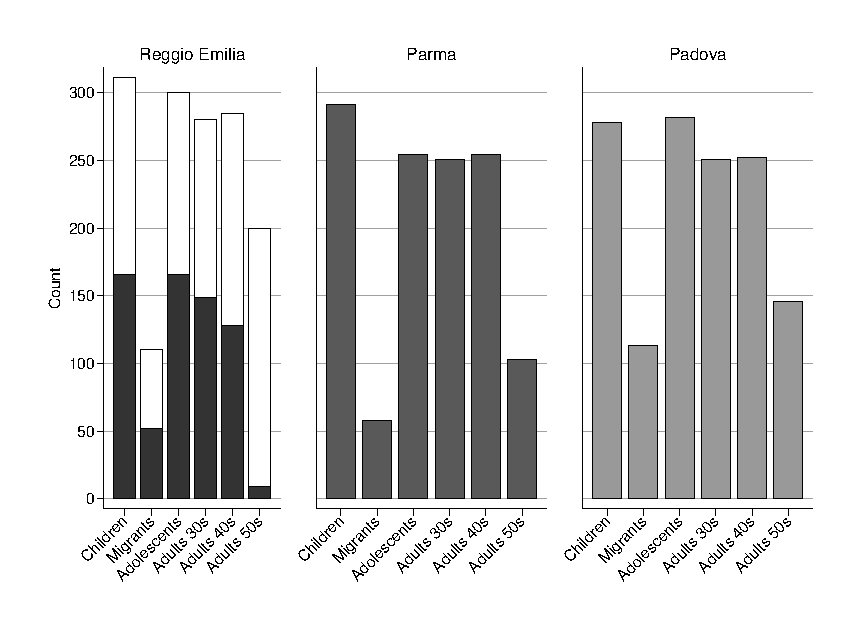
\includegraphics[width=.9\textwidth]{output/sample.eps}
\end{center}
\footnotetext{\noindent Note: This figure displays the number of individuals by cohort and city. The bars for Reggio Emilia differentiate between those who attended municipal preschool (black bars) and those who did not (white bars). Those in Reggio Emilia who attended municipal preschools are considered the treatment group.}
\end{figure}

\begin{table}[H]
\centering
\scalebox{0.7}{
\begin{threeparttable}
	\caption{The Sample by Cohort, City, and School Type}\label{tab:sample}
	\begin{tabular}{l*{15}{c}}
\toprule
            &\mc{5}{c}{Reggio Emilia: 1,471}   &     \mc{5}{c}{ Parma: 1,198}       &      \mc{5}{c}{Padova: 1,305}      \\
           \cmidrule(lr){2-6} \cmidrule(lr){7-11} \cmidrule(lr){12-16} 
      &        None&       Muni.&       State&      Relig.&       Priv.&        None&       Muni.&       State&      Relig.&       Priv.&        None&       Muni.&       State&      Relig.&       Priv.\\
\midrule
Children    &           2&         166&          45&          92&           5&           6&         154&          43&        77&           9&           2&          82&          40&         141&          12\\
Migrants    &           4&          52&          37&          14&           1&           4&          35&          10&          	3&           6&           5&          36&          47&          23&           1\\
Adolescents &           7&         166&          22&          96&           6&           4&         116&          43&     82&           6&           1&          93&          47&         131&           6\\
Adults 30    &          57&         149&          31&          40&           1&          44&          98&          51&        50&          5&       47&         35&         26&            140&    1 \\
Adults 40    &          80&         128&          17&          52&           5&         116&          52&          26&       55&          1&        75&      27 &            24&            123&   \\
Adults 50    &         147&           9&          10&          28&           2&          72&          12&           7&          11&            &        57&      11 &           2 &           68&    2 \\
\midrule
	       &         297&         670&         162&         322&          20&         246&         467&   180&    278&          27&      187&      284 &            186&        626& 22  \\
\bottomrule
\end{tabular}


\begin{tablenotes}
Note: This table shows the sample size by city, cohort, and school type. These numbers do not include individuals with an unidentified preschool type. In total, there are 45 individuals with unidentified preschool type. We separate migrants and children for clarity in this table even though they are in the same birth cohort (year of birth: 2006). None: no preschool; Muni.: municipal preschool;  State: state preschool; Relig.: religious preschool; Priv.: private preschool.
\end{tablenotes}
\end{threeparttable}
}
\end{table}

The structure of the cohorts allows us to study the effects of the Reggio Approach at different points throughout the life cycle. The youngest cohort of children were interviewed when they entered primary school, the adolescent cohort when they ended compulsory schooling, and the adult cohorts capture different points of adulthood to measure key outcomes such as engagement in the labor market, health, and family decisions. This cohort structure also allows us to evaluate the Reggio Approach compared to the alternative early childhood experiences as they evolved over time.

Separate questionnaires were administered to the children, adolescents, and adults, as well as to the caregivers of the children and adolescents. The questionnaires included items about early childhood experiences, family structure, education, interaction with non-Italians (or with Italians in the case of the migrant children), and measures of cognitive and social-emotional skills. The questionnaires for adults additionally included items about occupation, income, and life satisfaction. 

\section{Basic Analysis}
\label{sec:methodology}

We present a basic specification of OLS to estimate the effect of the Reggio Approach on an outcome of interest, $Y$, compared to not attending preschool at all. For this abbreviated analysis, we restrict to individuals from Reggio Emilia who either attended a Reggio Approach preschool or did not attend any preschool (across all cohorts, $N = 967$).

For individual $i$ in Reggio Emilia, let $\mu_i$ indicate whether that individual attended a Reggio Approach preschool. We select a vector, $\bm{X}_i$, of five baseline control variables with the lowest BIC to account for family background.\footnote{These variables are: \color{maroon}{forthcoming}} For each cohort, we estimate $\beta_1$ in the simple model

\begin{equation}
	Y_i = \beta_0 + \beta_1 \mu_i + \bm{X}_i\bm{\beta} + \varepsilon_i
	\label{eq:ra-v-none}
\end{equation}

\noindent where we $\varepsilon_i$ is a random disturbance. 

While this estimate is useful in gaining a basic understanding of the effect of the Reggio Approach, there is a clear selection issue. That is, the choice to enroll a child in the Reggio Approach and the choice to not enroll a child in any preschool are likely tied to family characteristics. After Section~\ref{sec:results} in which we present the estimates from Equation~\eqref{eq:ra-v-none}, we present a discussion of selection on observed characteristics.

\subsection{Results}
\label{sec:results}



Tables \ref{ols-E-reg} to \ref{ols-S-reg} show the OLS estimates of the effect of the Reggio Approach preschools for people in Reggio Emilia who attended Reggio Approach preschools compared to those who did not attend preschool at all. We do not include the age-50 cohort in this analysis, as the Reggio Approach did not exist for that cohort. We perform analysis using (i) no control, (ii) 6 controls selected by Bayesian Information Criterion (BIC), and (iii) the full set of controls that include baseline variables available for the adult cohorts. 

Table \ref{ols-E-reg} shows statistically significant effects of the Reggio Approach on high school grade for age-30 cohort. However, it should be noted that the high school grade measure in the data is not standardized across different schools. 


\begin{table}[H] \caption{OLS Results for Cognitive and Education, Municipal vs. None, Reggio Emilia} \label{ols-E-reg}
{
\def\sym#1{\ifmmode^{#1}\else\(^{#1}\)\fi}
\begin{tabular}{l*{6}{c}}
\toprule
            &\multicolumn{1}{c}{(1)}&\multicolumn{1}{c}{(2)}&\multicolumn{1}{c}{(3)}&\multicolumn{1}{c}{(4)}&\multicolumn{1}{c}{(5)}&\multicolumn{1}{c}{(6)}\\
            &\multicolumn{1}{c}{None30}&\multicolumn{1}{c}{BIC30}&\multicolumn{1}{c}{Full30}&\multicolumn{1}{c}{None40}&\multicolumn{1}{c}{BIC40}&\multicolumn{1}{c}{Full40}\\
\midrule
IQ Factor   &     0.00406         &      -0.220         &      -0.293         &     -0.0747         &     -0.0638         &      -0.162         \\
            &     (0.149)         &     (0.156)         &     (0.161)         &     (0.120)         &     (0.142)         &     (0.170)         \\
\addlinespace
High School Grade&       4.051\sym{*}  &       5.042\sym{*}  &       3.969         &       0.690         &       2.034         &       1.398         \\
            &     (1.961)         &     (2.130)         &     (2.401)         &     (1.395)         &     (1.618)         &     (2.232)         \\
\addlinespace
University Grade&       2.390         &      0.0387         &       0.638         &      -0.826         &      -0.222         &      -1.926         \\
            &     (2.233)         &     (2.552)         &     (2.840)         &     (2.433)         &     (2.751)         &     (5.638)         \\
\addlinespace
Graduate from High School&     -0.0424         &      0.0301         &     0.00954         &      -0.170\sym{***}&     -0.0525         &     -0.0315         \\
            &    (0.0502)         &    (0.0495)         &    (0.0577)         &    (0.0502)         &    (0.0542)         &    (0.0669)         \\
\addlinespace
Max Edu: University&      -0.120         &     -0.0673         &     -0.0744         &     -0.0188         &      0.0528         &      0.0572         \\
            &    (0.0670)         &    (0.0684)         &    (0.0716)         &    (0.0535)         &    (0.0608)         &    (0.0624)         \\
\addlinespace
Max Edu: Graduate School&     0.00671         &     0.00747         &     0.00700         &           0         &           0         &           0         \\
            &   (0.00672)         &   (0.00769)         &   (0.00744)         &         (.)         &         (.)         &         (.)         \\
\bottomrule
\end{tabular}
}

\vspace{1ex} \\
\footnotesize\raggedright{Note: This table shows the OLS estimates for attending Reggio Approach schools for people in Reggio Emilia who attended Reggio Approach preschools or no preschool at all. Column title indicates the age group and control set used in each regression corresponding to the column. ``None30'' refers to the regression with only age-30 cohort and with no control variables. ``BIC30'' refers to the regression with only age-30 cohort and with controls selected by Bayesian Information Criterion (BIC). ``Full30'' refers to the regression with only age-30 cohort and with the full set of controls. Analogous meanings applied to the age-40 cohort. Robust standard errors are reported in parentheses. Stars show statistical significance as follows. * p < 0.05, ** p < 0.01, *** p < 0.001.}
\end{table}

Table \ref{ols-W-reg} shows consistently significant positive effects of the Reggio Approach on hours worked per week. Moreover, there are significant effects on the indicator for the lowest household income category for the age-40 cohort. Note that the measures for subject labor income, including ``Monthly Wage'' presented in the table, have very few observations. Household income suffers less from the missing value problem.

\begin{table}[H] \caption{OLS Results for Employment and Income, Municipal vs. None, Reggio Emilia} \label{ols-W-reg}
\scalebox{0.92}{
{
\def\sym#1{\ifmmode^{#1}\else\(^{#1}\)\fi}
\begin{tabular}{l*{6}{c}}
\toprule
            &\multicolumn{1}{c}{(1)}&\multicolumn{1}{c}{(2)}&\multicolumn{1}{c}{(3)}&\multicolumn{1}{c}{(4)}&\multicolumn{1}{c}{(5)}&\multicolumn{1}{c}{(6)}\\
            &\multicolumn{1}{c}{None30}&\multicolumn{1}{c}{BIC30}&\multicolumn{1}{c}{Full30}&\multicolumn{1}{c}{None40}&\multicolumn{1}{c}{BIC40}&\multicolumn{1}{c}{Full40}\\
\midrule
Employed    &      0.0717         &      0.0526         &      0.0588         &      0.0652         &      0.0574\sym{*}  &    -0.00160         \\
            &    (0.0435)         &    (0.0432)         &    (0.0458)         &    (0.0348)         &    (0.0287)         &    (0.0356)         \\
\addlinespace
Self-Employed&     -0.0566         &      -0.102         &     -0.0994         &      0.0461         &      0.0126         &     0.00948         \\
            &    (0.0591)         &    (0.0631)         &    (0.0686)         &    (0.0487)         &    (0.0556)         &    (0.0763)         \\
\addlinespace
Hours Worked Per Week&       6.476\sym{**} &       6.134\sym{**} &       6.180\sym{**} &       4.736\sym{*}  &       3.648         &       4.713\sym{*}  \\
            &     (1.987)         &     (2.110)         &     (2.028)         &     (1.880)         &     (1.891)         &     (2.354)         \\
\addlinespace
Monthly Wage&      -188.4\sym{*}  &      -179.1\sym{*}  &      -192.6         &      -849.4         &     -1088.6         &       243.9         \\
            &     (74.31)         &     (88.37)         &     (118.0)         &     (699.5)         &     (758.5)         &    (1080.8)         \\
\addlinespace
Income: 5,000 Euros of Less&       0.148\sym{***}&       0.157\sym{***}&       0.173\sym{***}&     -0.0125         &    -0.00656         &     -0.0134         \\
            &    (0.0292)         &    (0.0350)         &    (0.0421)         &    (0.0125)         &   (0.00635)         &    (0.0133)         \\
\addlinespace
Income: 5,001-10,000 Euros&     -0.0284         &     -0.0220         &     -0.0278         &           0         &           0         &           0         \\
            &    (0.0254)         &    (0.0249)         &    (0.0246)         &         (.)         &         (.)         &         (.)         \\
\addlinespace
Income: 10,001-25,000 Euros&      -0.199\sym{**} &      -0.158         &      -0.217\sym{*}  &     -0.0531         &     -0.0284         &     -0.0338         \\
            &    (0.0760)         &    (0.0838)         &    (0.0897)         &    (0.0672)         &    (0.0728)         &    (0.0896)         \\
\addlinespace
Income: 25,001-50,000 Euros&      0.0741         &      0.0332         &      0.0728         &      0.0797         &      0.0464         &     -0.0259         \\
            &    (0.0780)         &    (0.0874)         &    (0.0882)         &    (0.0707)         &    (0.0754)         &    (0.0930)         \\
\addlinespace
Income: 50,001-100,000 Euros&     0.00518         &    -0.00974         &   -0.000807         &      0.0250         &      0.0365         &      0.0525         \\
            &    (0.0294)         &    (0.0306)         &    (0.0214)         &    (0.0303)         &    (0.0340)         &    (0.0317)         \\
\addlinespace
Income: 100,001-250,000 Euros&           0         &           0         &           0         &     -0.0391         &     -0.0479         &      0.0205         \\
            &         (.)         &         (.)         &         (.)         &    (0.0303)         &    (0.0299)         &    (0.0335)         \\
\addlinespace
Income: More than 250,000 Euros&           0         &           0         &           0         &           0         &           0         &           0         \\
            &         (.)         &         (.)         &         (.)         &         (.)         &         (.)         &         (.)         \\
\bottomrule
\end{tabular}
}
}
\vspace{1ex} \\
\footnotesize\raggedright{Note: This table shows the OLS estimates for attending Reggio Approach schools for people in Reggio Emilia who attended Reggio Approach preschools or no preschool at all. Column title indicates the age group and control set used in each regression corresponding to the column. ``None30'' refers to the regression with only age-30 cohort and with no control variables. ``BIC30'' refers to the regression with only age-30 cohort and with controls selected by Bayesian Information Criterion (BIC). ``Full30'' refers to the regression with only age-30 cohort and with the full set of controls. Analogous meanings applied to the age-40 cohort. Robust standard errors are reported in parentheses. Stars show statistical significance as follows. * p < 0.05, ** p < 0.01, *** p < 0.001.}
\end{table}

Table \ref{ols-L-reg} shows significant effects of the Reggio Approach on the status of being divorced for the age-30 cohort. Other results do not show any significant trend. 

\begin{table}[H] \caption{OLS Results for Living Environment, Municipal vs. None, Reggio Emilia} \label{ols-L-reg}
{
\def\sym#1{\ifmmode^{#1}\else\(^{#1}\)\fi}
\begin{tabular}{l*{6}{c}}
\toprule
            &\multicolumn{1}{c}{(1)}&\multicolumn{1}{c}{(2)}&\multicolumn{1}{c}{(3)}&\multicolumn{1}{c}{(4)}&\multicolumn{1}{c}{(5)}&\multicolumn{1}{c}{(6)}\\
            &\multicolumn{1}{c}{None30}&\multicolumn{1}{c}{BIC30}&\multicolumn{1}{c}{Full30}&\multicolumn{1}{c}{None40}&\multicolumn{1}{c}{BIC40}&\multicolumn{1}{c}{Full40}\\
\midrule
Married or Cohabitating&      0.0652         &     -0.0665         &     -0.0129         &     0.00781         &     -0.0164         &      0.0201         \\
            &    (0.0754)         &    (0.0810)         &    (0.0827)         &    (0.0618)         &    (0.0703)         &    (0.0965)         \\
\addlinespace
Divorced    &      0.0268\sym{*}  &      0.0409\sym{*}  &      0.0192         &     -0.0312         &     -0.0113         &      0.0373         \\
            &    (0.0133)         &    (0.0204)         &    (0.0130)         &    (0.0453)         &    (0.0478)         &    (0.0615)         \\
\addlinespace
Num. of Children in House&      0.0223         &      0.0172         &      0.0418         &      0.0563         &     -0.0530         &     -0.0707         \\
            &    (0.0519)         &    (0.0566)         &    (0.0603)         &    (0.0846)         &    (0.0979)         &     (0.106)         \\
\addlinespace
Own House   &    -0.00177         &      0.0830         &       0.153         &     -0.0859         &     -0.0160         &     -0.0294         \\
            &    (0.0773)         &    (0.0845)         &    (0.0899)         &    (0.0642)         &    (0.0707)         &    (0.0812)         \\
\addlinespace
Live With Parents&     -0.0613         &      -0.102         &     -0.0876         &     -0.0266         &     -0.0375         &     -0.0413         \\
            &    (0.0570)         &    (0.0531)         &    (0.0544)         &    (0.0279)         &    (0.0254)         &    (0.0297)         \\
\bottomrule
\end{tabular}
}

\vspace{1ex} \\
\footnotesize\raggedright{Note: This table shows the OLS estimates for attending Reggio Approach schools for people in Reggio Emilia who attended Reggio Approach preschools or no preschool at all. Column title indicates the age group and control set used in each regression corresponding to the column. ``None30'' refers to the regression with only age-30 cohort and with no control variables. ``BIC30'' refers to the regression with only age-30 cohort and with controls selected by Bayesian Information Criterion (BIC). ``Full30'' refers to the regression with only age-30 cohort and with the full set of controls. Analogous meanings applied to the age-40 cohort. Robust standard errors are reported in parentheses. Stars show statistical significance as follows. * p < 0.05, ** p < 0.01, *** p < 0.001.}
\end{table}

Table \ref{ols-H-reg} show that the significantly increasing effects of the Reggio Approach on numbers of days sick for the past month at the time of the interview for the age-30 cohort. Moreover, the results show the significant decreasing effects on whether the respondent has ever been suspended from school. 

\begin{table}[H] \caption{OLS Results for Health, Municipal vs. None, Reggio Emilia} \label{ols-H-reg}
{
\def\sym#1{\ifmmode^{#1}\else\(^{#1}\)\fi}
\begin{tabular}{l*{2}{c}}
\hline\hline
            &\multicolumn{1}{c}{(1)}&\multicolumn{1}{c}{(2)}\\
            &\multicolumn{1}{c}{Muni30}&\multicolumn{1}{c}{Muni40}\\
\hline
Tried Marijuana&      0.0916         &      0.0864         \\
            &    (0.0563)         &    (0.0507)         \\
[1em]
Smokes      &           0         &           0         \\
            &         (.)         &         (.)         \\
[1em]
Num. of Cigarettes Per Day&       2.431         &      -0.372         \\
            &     (1.348)         &     (1.666)         \\
[1em]
BMI         &       0.620         &      -0.220         \\
            &     (0.412)         &     (0.482)         \\
[1em]
Good Health &       0.129         &       0.126         \\
            &    (0.0775)         &     (0.103)         \\
[1em]
Num. of Days Sick Past Month&       0.285\sym{***}&      0.0400         \\
            &    (0.0848)         &    (0.0872)         \\
[1em]
Engaged in A Fight&           0         &           0         \\
            &         (.)         &         (.)         \\
[1em]
Drove Under Influence&           0         &           0         \\
            &         (.)         &         (.)         \\
[1em]
Ever Suspended from School&      -0.141\sym{**} &     -0.0159         \\
            &    (0.0521)         &    (0.0545)         \\
[1em]
Age At First Drink&      -0.518         &      -0.367         \\
            &     (1.238)         &     (1.396)         \\
\hline\hline
\multicolumn{3}{l}{\footnotesize \specialcell{\underline{Note:} This table shows the OLS estimates for people in Reggio who attended municipal preschools or none. \\                                                                         Standard errors are reported in parenthesis. Stars show statistical significance as follows: \\                                                                         * p < 0.05, ** p < 0.01, *** p < 0.001.}}\\
\end{tabular}
}

\vspace{1ex} \\
\footnotesize\raggedright{Note: This table shows the OLS estimates for attending Reggio Approach schools for people in Reggio Emilia who attended Reggio Approach preschools or no preschool at all. Column title indicates the age group and control set used in each regression corresponding to the column. ``None30'' refers to the regression with only age-30 cohort and with no control variables. ``BIC30'' refers to the regression with only age-30 cohort and with controls selected by Baysian Information Criterion (BIC). ``Full30'' refers to the regression with only age-30 cohort and with the full set of controls. Analogous meanings applied to the age-40 cohort. Robust standard errors are reported in parentheses. Stars show statistical significance as follows. * p < 0.05, ** p < 0.01, *** p < 0.001.}
\end{table}

Table \ref{ols-N-reg} shows no consistently significant trends between the age-30 cohort and age-40 cohort. For the age-30 cohort, there are significantly decreasing effects on the optimistic look in life. Moreover, there are significantly increasing effects on whether the respondent is likely to do the same to someone who puts him/her in a difficult situation and to someone who insults him/her.

For the age-40 cohort, results show the significantly decreasing effects on depression for the age-30 cohort. There are also significantly positive effects on satisfaction with income and with work for the age-40 cohort. However, there are significantly positive effects on whether the respondent thinks work is source of stress. 

\begin{table}[H] \caption{OLS Results for Non-cognitive, Municipal vs. None, Reggio Emilia} \label{ols-N-reg}
{
\def\sym#1{\ifmmode^{#1}\else\(^{#1}\)\fi}
\begin{tabular}{l*{6}{c}}
\toprule
            &\multicolumn{1}{c}{(1)}&\multicolumn{1}{c}{(2)}&\multicolumn{1}{c}{(3)}&\multicolumn{1}{c}{(4)}&\multicolumn{1}{c}{(5)}&\multicolumn{1}{c}{(6)}\\
            &\multicolumn{1}{c}{None30}&\multicolumn{1}{c}{BIC30}&\multicolumn{1}{c}{Full30}&\multicolumn{1}{c}{None40}&\multicolumn{1}{c}{BIC40}&\multicolumn{1}{c}{Full40}\\
\midrule
Locus of Control - positive&      0.0713         &      -0.133         &      -0.122         &       0.171         &       0.162         &       0.199         \\
            &     (0.127)         &     (0.125)         &     (0.127)         &     (0.119)         &     (0.137)         &     (0.165)         \\
\addlinespace
Depression Score - positive&       1.337         &      -0.678         &      -0.251         &       2.399\sym{**} &       1.848         &       2.225\sym{*}  \\
            &     (0.920)         &     (0.849)         &     (0.883)         &     (0.872)         &     (0.962)         &     (1.085)         \\
\addlinespace
Stress      &       0.184         &       0.102         &      0.0645         &       0.255\sym{*}  &       0.201         &       0.134         \\
            &     (0.111)         &     (0.108)         &     (0.126)         &     (0.104)         &     (0.112)         &     (0.150)         \\
\addlinespace
Work is Source of Stress&      0.0933         &      0.0639         &      0.0222         &       0.162         &       0.179\sym{*}  &       0.249\sym{*}  \\
            &    (0.0994)         &     (0.102)         &    (0.0983)         &    (0.0857)         &    (0.0882)         &     (0.101)         \\
\addlinespace
Satisfied with Income&       0.240         &       0.272         &       0.221         &       0.269\sym{*}  &       0.300\sym{*}  &       0.306         \\
            &     (0.142)         &     (0.153)         &     (0.152)         &     (0.128)         &     (0.147)         &     (0.161)         \\
\addlinespace
Satisfied with Work&       0.122         &       0.126         &       0.125         &       0.353\sym{**} &       0.315\sym{**} &       0.248         \\
            &     (0.138)         &     (0.149)         &     (0.146)         &     (0.114)         &     (0.122)         &     (0.145)         \\
\addlinespace
Satisfied with Health&     -0.0871         &      -0.180         &      -0.191         &      0.0578         &      0.0169         &    0.000877         \\
            &     (0.108)         &     (0.110)         &     (0.135)         &    (0.0700)         &    (0.0857)         &     (0.102)         \\
\addlinespace
Satisfied with Family&      0.0616         &     -0.0277         &      0.0122         &       0.227\sym{*}  &       0.142         &      0.0969         \\
            &     (0.134)         &     (0.143)         &     (0.148)         &     (0.116)         &     (0.137)         &     (0.157)         \\
\addlinespace
Optimistic Look in Life&      -0.173\sym{*}  &      -0.197\sym{*}  &      -0.127         &     -0.0632         &    -0.00647         &       0.105         \\
            &    (0.0746)         &    (0.0771)         &    (0.0874)         &    (0.0716)         &    (0.0816)         &     (0.108)         \\
\addlinespace
Return Favor&      0.0610         &     -0.0535         &     -0.0901         &      0.0891         &     0.00774         &     -0.0505         \\
            &     (0.159)         &     (0.154)         &     (0.192)         &     (0.128)         &     (0.149)         &     (0.195)         \\
\addlinespace
Put Someone in Difficulty&       0.615\sym{***}&       0.688\sym{***}&       0.642\sym{**} &      0.0109         &      -0.119         &       0.154         \\
            &     (0.178)         &     (0.191)         &     (0.205)         &     (0.163)         &     (0.191)         &     (0.213)         \\
\addlinespace
Help Someone Kind To Me&     -0.0164         &     -0.0848         &      -0.146         &       0.102         &      0.0696         &     0.00196         \\
            &     (0.111)         &     (0.110)         &     (0.123)         &    (0.0940)         &    (0.0977)         &     (0.124)         \\
\addlinespace
Insult Back &       0.387\sym{*}  &       0.524\sym{**} &       0.719\sym{***}&      -0.369\sym{*}  &      -0.272         &     -0.0920         \\
            &     (0.176)         &     (0.169)         &     (0.169)         &     (0.158)         &     (0.164)         &     (0.209)         \\
\bottomrule
\end{tabular}
}

\vspace{1ex} \\
\footnotesize\raggedright{Note: This table shows the OLS estimates for attending Reggio Approach schools for people in Reggio Emilia who attended Reggio Approach preschools or no preschool at all. Column title indicates the age group and control set used in each regression corresponding to the column. ``None30'' refers to the regression with only age-30 cohort and with no control variables. ``BIC30'' refers to the regression with only age-30 cohort and with controls selected by Bayesian Information Criterion (BIC). ``Full30'' refers to the regression with only age-30 cohort and with the full set of controls. Analogous meanings applied to the age-40 cohort. Robust standard errors are reported in parentheses. Stars show statistical significance as follows. * p < 0.05, ** p < 0.01, *** p < 0.001.}
\end{table}

Table \ref{ols-S-reg} shows consistently significant and negative effects of the Reggio Approach on whether the respondent does volunteer work for both the age-30 and age-40 cohorts. Moreover, for the age-40 cohort, there are significantly negative effects on respondents having migrant friends and significantly positive effects on whether respondents have ever voted for municipal and regional elections. For the age-30 cohort, there are significantly negative effects on whether respondents have ever voted for national elections.

\begin{table}[H] \caption{OLS Results for Social Behavior, Municipal vs. None, Reggio Emilia} \label{ols-S-reg}
{
\def\sym#1{\ifmmode^{#1}\else\(^{#1}\)\fi}
\begin{tabular}{l*{6}{c}}
\toprule
            &\multicolumn{1}{c}{(1)}&\multicolumn{1}{c}{(2)}&\multicolumn{1}{c}{(3)}&\multicolumn{1}{c}{(4)}&\multicolumn{1}{c}{(5)}&\multicolumn{1}{c}{(6)}\\
            &\multicolumn{1}{c}{None30}&\multicolumn{1}{c}{BIC30}&\multicolumn{1}{c}{Full30}&\multicolumn{1}{c}{None40}&\multicolumn{1}{c}{BIC40}&\multicolumn{1}{c}{Full40}\\
\midrule
Favorable to Migrants&      -0.070         &      -0.062         &       -0.12         &     -0.0078         &       0.027         &      -0.013         \\
            &      (0.08)         &      (0.09)         &      (0.10)         &      (0.09)         &      (0.09)         &      (0.12)         \\
\addlinespace
Number of Friends&       -1.46         &       -1.41         &       -1.53         &       -2.07\sym{*}  &       -0.82         &        0.13         \\
            &      (1.36)         &      (1.66)         &      (1.55)         &      (0.92)         &      (0.94)         &      (1.47)         \\
\addlinespace
Has Migrant Friends&       0.041         &       0.044         &     -0.0055         &       -0.13\sym{*}  &       -0.11         &       -0.18\sym{*}  \\
            &      (0.07)         &      (0.07)         &      (0.08)         &      (0.06)         &      (0.07)         &      (0.09)         \\
\addlinespace
Volunteers  &       -0.15\sym{**} &       -0.15\sym{**} &       -0.16\sym{**} &       -0.15\sym{**} &      -0.088         &       -0.21\sym{**} \\
            &      (0.06)         &      (0.05)         &      (0.06)         &      (0.05)         &      (0.06)         &      (0.08)         \\
\addlinespace
Child Eats Meal with Fam&        0.33         &      -0.096         &       0.011         &       0.095         &       0.078         &        0.13         \\
            &      (0.21)         &      (0.17)         &      (0.25)         &      (0.14)         &      (0.15)         &      (0.20)         \\
\addlinespace
Ever Voted for Municipal&        0.27\sym{***}&        0.11         &        0.11         &        0.30\sym{***}&       0.099         &        0.18\sym{*}  \\
            &      (0.08)         &      (0.06)         &      (0.07)         &      (0.07)         &      (0.08)         &      (0.08)         \\
\addlinespace
Ever Voted for Regional&        0.21\sym{**} &       0.099         &       0.088         &        0.30\sym{***}&        0.12         &        0.23\sym{**} \\
            &      (0.08)         &      (0.07)         &      (0.08)         &      (0.07)         &      (0.08)         &      (0.09)         \\
\addlinespace
Ever Voted for National&       -0.10\sym{*}  &       -0.13\sym{**} &      -0.090         &       0.094         &       0.030         &       0.078         \\
            &      (0.05)         &      (0.05)         &      (0.05)         &      (0.06)         &      (0.06)         &      (0.08)         \\
\bottomrule
\end{tabular}
}

\vspace{1ex} \\
\footnotesize\raggedright{Note: This table shows the OLS estimates for attending Reggio Approach schools for people in Reggio Emilia who attended Reggio Approach preschools or no preschool at all. Column title indicates the age group and control set used in each regression corresponding to the column. ``None30'' refers to the regression with only age-30 cohort and with no control variables. ``BIC30'' refers to the regression with only age-30 cohort and with controls selected by Bayesian Information Criterion (BIC). ``Full30'' refers to the regression with only age-30 cohort and with the full set of controls. Analogous meanings applied to the age-40 cohort. Robust standard errors are reported in parentheses. Stars show statistical significance as follows. * p < 0.05, ** p < 0.01, *** p < 0.001.}
\end{table}




\section{Discussion of Selection}
\label{sec:selection}

The selection into preschool, as well as the selection into a particular type of preschool, might be determined by social, demographic, and economic characteristics of the family. Some of these characteristics might be observed in our data, and other might be omitted. We begin our exploration of the selection on observed characteristics by presenting the distributions of parental education.

Figures~\ref{fig:momEdu} and~\ref{fig:dadEdu} present the distribution of parental educational attainment for individuals from each combination of city, cohort, and preschool type. Figure~\ref{fig:momEdu} shows that within Reggio Emilia, mothers of individuals who did not attend preschool have proportionally higher levels of high school and university education than mothers of individuals who attended some form of preschool. This difference is more pronounced for the older cohorts. Figure~\ref{fig:dadEdu} shows that a similar pattern persists when examining father's education. A clear pattern does not emerge when we compare parental educational attainment between individuals who attended different types of preschool in Reggio Emilia. This suggests that parental education might have played a larger role in the initial decision of sending an individual to preschool, as compared to the subsequent decision of choosing a particular type of preschool. Figures~\ref{fig:momEdu} and~\ref{fig:dadEdu} include analogous graphs for Parma and Padova.

Figure~\ref{fig:parentsEdu} examines the difference of educational attainment between mothers and fathers for individuals from each city-cohort combination. Each column represents the total proportion of individuals in each city-cohort combination whose fathers are more educated than mothers. Each column is further broken down into sections that calculate this proportion conditional on different levels of father's education. The figures show that total inequality in educational attainment is largest in Padova and smallest in Reggio Emilia, and that this ranking of total inequality is consistent across the three adult cohorts. Furthermore, for the older cohorts, the level of inequality is substantially larger in Padova compared to Reggio Emilia and Parma. Padova is similar to the other two cities by the time we reach the age 30 cohort. 


\begin{figure}[!htb]
	\begin{minipage}{1\textwidth}
	\centering
	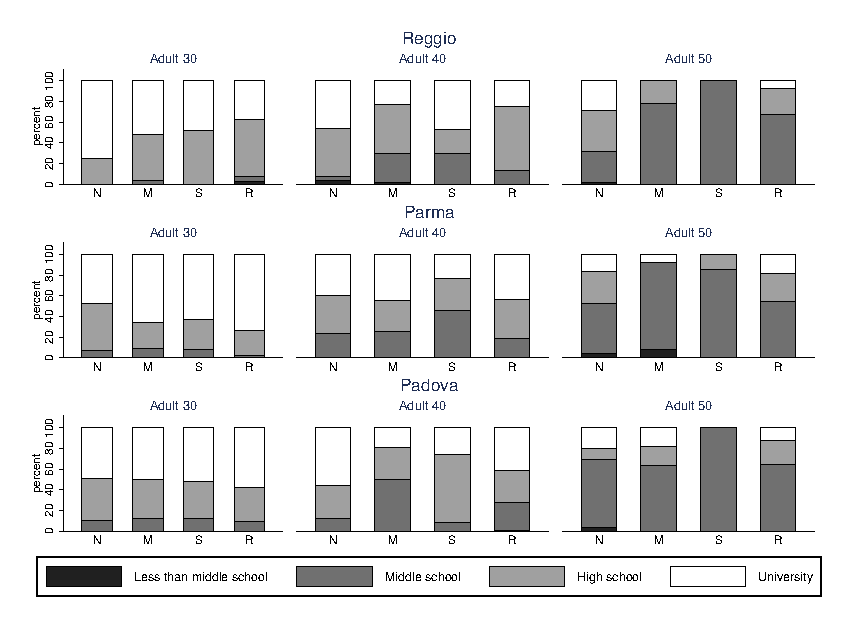
\includegraphics[scale=1.2]{../../Output/image/bar_momEdu}
	\caption{Mother's educational attainment by city, cohort and materna type}
	\label{fig:momEdu}
	\footnotetext{Note:  \textbf{(1)} Definiteion of bar labels: N = Not attended; M = Municipal; S = State; R = Religious. \textbf{(2)} Each bar presents the distribution of mothers' educational attainment for individuals in each city-cohort-materna type combination. }
	\end{minipage}
\end{figure}

\begin{figure}[!htb]
	\begin{minipage}{1\textwidth}
	\centering
	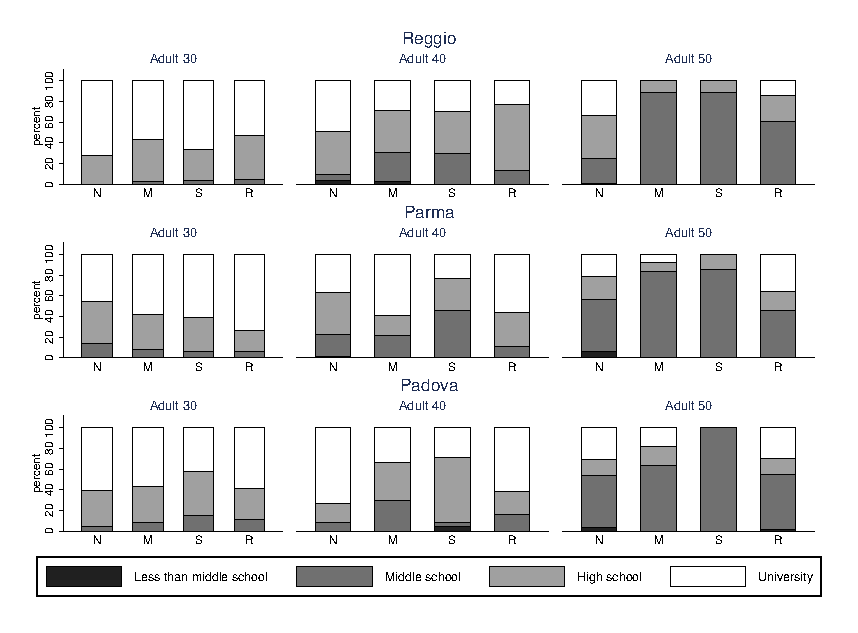
\includegraphics[scale=1.2]{../../Output/image/bar_dadEdu}
	\caption{Father's education attainment by city, cohort and materna type}
	\label{fig:dadEdu}
	\footnotetext{Note:  \textbf{(1)} Definiteion of bar labels: N = Not attended; M = Municipal; S = State; R = Religious. \textbf{(2)} Each bar presents the distribution of fathers' educational attainment for individuals in each city-cohort-materna type combination. }
	\end{minipage}
\end{figure}

\begin{figure}[!htb]
	\begin{minipage}{.9\textwidth}
	\centering
	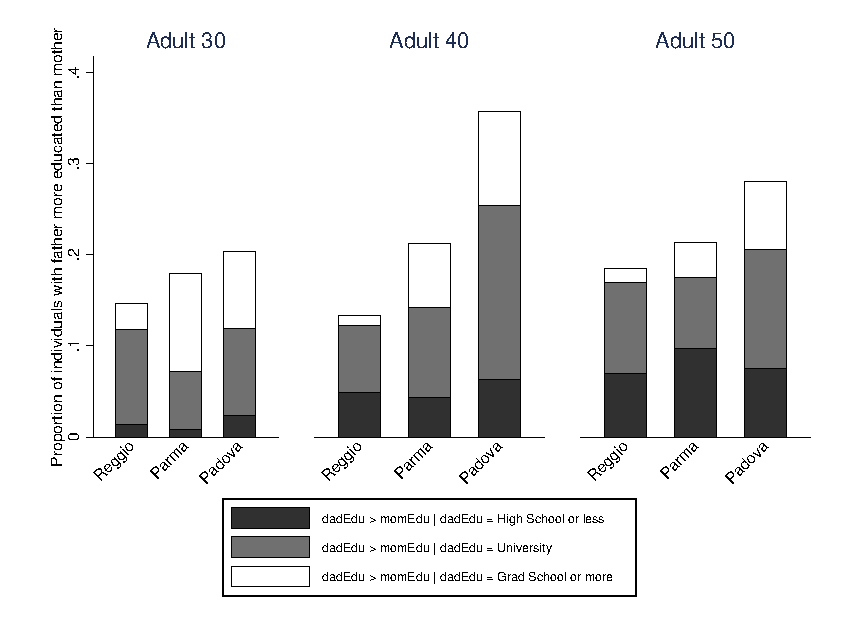
\includegraphics[scale=1]{../../Output/image/bar_parentsEduCompare}
	\caption{Proportion of individuals with fathers who are more educated than mothers by city and cohort}
	\label{fig:parentsEdu}
	\footnotetext{\noindent Note: Each column represents the proportion of individuals within each city-cohort combination whose fathers were more educated than their mothers.}
	\end{minipage}
\end{figure}

\clearpage

\bibliography{heckman}
\bibliographystyle{chicago}

\end{document}
